\section{Angular cancellation and all-time approximation}\label{sec:angular}

We now fix the transports $U_e$ and component matrices $T_i$, and
restrict the initial finite tuple to the ball supplied by
Theorem~\ref{thm:finite-force}. In addition to the energy bounds of
Section~\ref{sec:reconstruction}, we then have
\begin{equation}\label{eq:integrable-forces}
 \int_0^\infty(F+V)\,ds\le C,\qquad
 \int_0^\infty\Phi(H(s))\,ds\le C.
\end{equation}
The constants may depend on the fixed constraint maps. We use the
same reconstructed metric $\widehat K$; the argument changes how
its residual is estimated.

\begin{proposition}\label{prop:global-weak-residual}
There are global complex endomorphism-valued one-forms $J(s)$
and integrable endomorphisms $B(s)$ such that
\begin{equation}\label{eq:global-weak-residual}
 \cR(\widehat K)=D^*J+B,\qquad
 \int_0^\infty\!\int_{C_\tau}|J|^2\le C\rho^2,\qquad
 \int_0^\infty\!\int_{C_\tau}|B|\le C a_*,
\end{equation}
where, for one fixed finite exponent $N$,
\begin{equation}\label{eq:all-time-error}
 a_*=\alpha_*+\epsilon_*\ell^2+b^2\rho^{-N}\longrightarrow0.
\end{equation}
The divergence identity is distributional on the closed fibre.
The forms $J$ are smooth on each incidence collar, have zero normal
trace on both boundary circles, and are extended by zero elsewhere.
Constants are independent of time and every ratio among the
component and node scales.
\end{proposition}

\subsection{A radial reference metric}
Consider an elliptic incidence collar
$A_\rho=\{\rho<|z|<2\rho\}$ in its parallel node frame. At the
current time keep the finite tuple, all weights and the corrected
node endpoints fixed. Introduce an auxiliary real variable $a$
and set
\[
 G_a(z)=e^{iaT_iF_{ie}(z)},\qquad
 \xi_i^{\mathrm{rad}}=-\epsilon_e B_{ij}\log|z|+c_{ie}.
\]
The variable $a$ is used only for a spatial Taylor expansion. It
does not change the trajectory or any parameter along that
trajectory. Define
\begin{equation}\label{eq:radial-family}
 K_a^{\mathrm{rad}}
 =H_i\exp\left((1-\chi)\log(H_i^{-1}N_e)
 +\chi\log\{H_i^{-1}G_a^*H_i e^{\xi_i^{\mathrm{rad}}}G_a\}\right).
\end{equation}
The metric $K_0^{\mathrm{rad}}$ is radial. The actual collar
metric is obtained at $a=\alpha_i$ by replacing
$\xi_i^{\mathrm{rad}}$ with $\xi_i^{\mathrm{rad}}+q_{ie}$.
No matrix factors have been commuted in this formula.

Write $\mathcal C(K)=2i\Lambda_\tau F_K$ for the spatial Chern
expression. Bounded derivatives of relative logarithms and
exponentials, together with \eqref{eq:regular-bounds}, imply
\begin{equation}\label{eq:regular-curvature-error}
 \int_{A_\rho}
   |\mathcal C(\widehat K)-\mathcal C(K_{\alpha_i}^{\mathrm{rad}})|
                        \,dA_\tau\le C\rho F_{\mathrm{ed}}.
\end{equation}
Indeed the change in each metric derivative of order $k\le2$ is
at most $CF_{\mathrm{ed}}\rho^{1-k}$. All other spatial inputs
have derivatives bounded by $C\rho^{-k}$. Substitution into the
full expression $-4a_\tau^{-1}\partial_{\bar z}(K^{-1}K_z)$
and multiplication by $dA_\tau$ give the asserted integral.
The quadratic error is smaller on the bounded range.

At $a=0$, comparison with the exactly flat node profile gives
\begin{equation}\label{eq:radial-curvature-error}
 \int_{A_\rho}|\mathcal C(K_0^{\mathrm{rad}})|\,dA_\tau
                   \le C\epsilon_*\ell^2F_{\mathrm{ed}}.
\end{equation}
Here is the endpoint expansion used in this estimate. At zero
regular endpoint corrections the relative node logarithm is
$\theta_e B_{ij}$, whereas at $\theta_e=0$ it is $c_{ie}$.
The difference from their sum therefore has size at most
$C\theta_e F_{\mathrm{ed}}$, with two spatial derivatives
bounded by the corresponding factors $\rho^{-1}$ and
$\rho^{-2}$. On the collar $\theta_e=O(\epsilon_e\ell)$.
In the curvature difference, the terms are bounded by
\[
 C\bigl(|\nabla^2\delta|+|\nabla n||\nabla\delta|
       +|\delta|(|\nabla^2n|+|\nabla n|^2)
       +|\nabla\delta|^2\bigr),
\]
where $n$ is the node logarithm. Its derivatives of positive
order are at most $C\epsilon_e\rho^{-k}$ on the bounded finite
ball. Integrating over the collar gives
\eqref{eq:radial-curvature-error}. All time derivatives of the
actual collar metric are bounded by $CV$; their residual integral
is at most $C\rho^2V$.

\subsection{The first variation has zero angular mean}
In a flat holomorphic frame with $dA_\tau=a_\tau(z)\,dx\,dy$,
\[
 \mathcal C(K)=-4a_\tau^{-1}
                         \partial_{\bar z}(K^{-1}\partial_z K).
\]
Put $K_0=K_0^{\mathrm{rad}}$,
$A_0=K_0^{-1}\partial_zK_0$ and
$W=K_0^{-1}\partial_a K_a^{\mathrm{rad}}|_{a=0}$.
The inverse derivative rule gives the exact variation
\begin{equation}\label{eq:chern-first-variation}
 \left.\partial_a\mathcal C(K_a^{\mathrm{rad}})\right|_0
  =-4a_\tau^{-1}\partial_{\bar z}
                       \{\partial_zW+[A_0,W]\}.
\end{equation}
All inputs of \eqref{eq:radial-family} except $G_a$ are radial.
Its first variation thus has the form
$W(z)=F_{ie}(z)W_0(|z|)$ for a radial matrix function $W_0$.
By \eqref{eq:primitive}, $W$ has only angular indices $1,-1$.

Multiplication of \eqref{eq:chern-first-variation} by
$a_\tau$ gives a rotationally invariant operator on the radial
background. To see the matrix order explicitly, set
$t=\log|z|$ and $C(t)=K_0^{-1}\partial_tK_0$. If
$W=e^{in\theta}w(t)$, direct differentiation gives
\begin{equation}\label{eq:polar-linearization}
 \begin{split}
 4\partial_{\bar z}\{\partial_zW+[A_0,W]\}
   =e^{-2t+in\theta}\bigl(&w''-n^2w+[C',w]\\
                       &+[C,w']-n[C,w]\bigr).
 \end{split}
\end{equation}
In particular each angular index is preserved, even when the
matrices fail to commute. Therefore the matrix-valued function
\begin{equation}\label{eq:angular-source}
 S_{ie}=a_\tau\alpha_i
       \left.\partial_a\mathcal C(K_a^{\mathrm{rad}})\right|_0
\end{equation}
has only the two indices $1,-1$, and
\begin{equation}\label{eq:zero-mean}
 \int_{A_\rho}S_{ie}\,dx\,dy=0
\end{equation}
entry by entry. The factor $a_\tau$ in
\eqref{eq:angular-source} is essential. We have not assumed
that the actual fibre metric is radial.

We next retain the force factors in this variation. For
$0\le k\le2$, uniformly between $a=0$ and $a=\alpha_i$,
\begin{equation}\label{eq:parameter-derivatives}
 \begin{split}
 |\nabla^k\partial_aK_a^{\mathrm{rad}}|
       &\le C\rho^{1-k}(m_i+\ell F_{\mathrm{ed}}),\\
 |\nabla^k\partial_a^2K_a^{\mathrm{rad}}|
       &\le C\rho^{2-k}(m_i+\ell F_{\mathrm{ed}}).
 \end{split}
\end{equation}
To prove these estimates, first differentiate
$G_a^*H_ie^{\xi_i^{\mathrm{rad}}}G_a$. Its first derivative is
$F_{ie}$ times a commutator with $iT_i$, and its second is
$F_{ie}^2$ times an iterated commutator. The matrix factors are
bounded by $C(m_i+|\xi_i^{\mathrm{rad}}|)$. Spatial derivatives
differentiate the linear harmonic function, the radial cutoff
or the radial logarithms. We have
$|\xi_i^{\mathrm{rad}}|\le C\ell F_{\mathrm{ed}}$ and
$|\nabla^k\xi_i^{\mathrm{rad}}|\le
CF_{\mathrm{ed}}\rho^{-k}$ for $k=1,2$.
The node logarithm has the same derivative bound because
$\epsilon_e(d_e+F_{\mathrm{ed}})\le CF_{\mathrm{ed}}$.
Composition with relative logarithms and exponentials preserves
these bounds. Products of two first parameter derivatives contain
$(m_i+\ell F_{\mathrm{ed}})^2$, which is bounded by a fixed
multiple of $m_i+\ell F_{\mathrm{ed}}$ on the finite ball.
This proves \eqref{eq:parameter-derivatives}, including when
$m_i=0$.

Using these estimates in the full Chern expression, with the
inverse-matrix derivatives in their stated order, gives
\begin{equation}\label{eq:source-norm}
 \|S_{ie}\|_{L^2(dx\,dy)}
       \le C|\alpha_i|(m_i+\ell F_{\mathrm{ed}}).
\end{equation}
Taylor's formula in $a$ also gives
\begin{equation}\label{eq:nonlinear-collar-remainder}
 \begin{split}
 \int_{A_\rho}\bigl|\mathcal C(K_{\alpha_i}^{\mathrm{rad}})
       -\mathcal C(K_0^{\mathrm{rad}})
       -\alpha_i\left.\partial_a\mathcal C(K_a^{\mathrm{rad}})
                                      \right|_0\bigr|\,dA_\tau
 \le C\alpha_i^2\rho^2(m_i+\ell F_{\mathrm{ed}}).
 \end{split}
\end{equation}
In each second parameter derivative of curvature there is either
one second metric variation or two first variations. Two spatial
derivatives in \eqref{eq:parameter-derivatives} bound both types.
The factor $a_\tau^{-1}$ cancels against area. Thus this estimate
includes the noncommuting quadratic terms, rather than estimating
only the scalar principal part.

\subsection{Neumann primitives on the actual bundle}
For each real and imaginary matrix entry solve
\begin{equation}\label{eq:neumann}
 -\Delta_{\RR^2}u_{ie}=S_{ie},\qquad
 \partial_nu_{ie}=0\ \text{on both boundary circles},\qquad
 \int_{A_\rho}u_{ie}\,dx\,dy=0.
\end{equation}
Equation \eqref{eq:zero-mean} is exactly the compatibility
condition. Minimizing the Dirichlet quadratic functional on
mean-zero $H^1$ functions proves existence and uniqueness.
Scaling the fixed annulus $\{1<|z|<2\}$ gives
$\|u\|_2\le C\rho\|du\|_2$. Testing \eqref{eq:neumann} by $u$
then gives
\begin{equation}\label{eq:neumann-energy}
 \|du_{ie}\|_{L^2(dx\,dy)}
                  \le C\rho\|S_{ie}\|_{L^2(dx\,dy)}.
\end{equation}

Set $J_{ie}=du_{ie}$ in the parallel node frame, and extend it
by zero outside the collar. In real dimension two,
$D^*=a_\tau^{-1}d_{\mathrm{Eucl}}^*$ in this frame. Testing
against a smooth global endomorphism and integrating on the
collar shows that its distributional divergence is precisely
$\alpha_i\partial_a\mathcal C(K_a^{\mathrm{rad}})|_0$ there
and zero elsewhere. There is no boundary measure, since the
normal component vanishes on both circles. Tangential jumps of
the extension do not enter divergence. Constant unitary changes
of node frame conjugate this construction and give a global
endomorphism-valued one-form.

Incidence collars are disjoint for sufficiently small parameters.
Their one-form energy is conformally invariant. Hence, for
$J=\sum_{ie}J_{ie}$,
\begin{equation}\label{eq:instantaneous-j}
 \begin{split}
 \int_{C_\tau}|J|^2
 &\le C\rho^2\sum_i\alpha_i^2
                   (m_i^2+\ell^2F_{\mathrm{ed}}^2)
 \le C\rho^2\Phi(H).
 \end{split}
\end{equation}
The last inequality follows from
\eqref{eq:force-energy-relations} and boundedness of
$\alpha_*^2\epsilon_*\ell^2$ for small joint parameters.
Rational incidences have $\alpha_i=0$ and require no primitive.
Each Neumann problem is on a fixed-shape collar. Its constant
does not depend on any of the long middle annuli.

\begin{figure}[htbp]
\centering
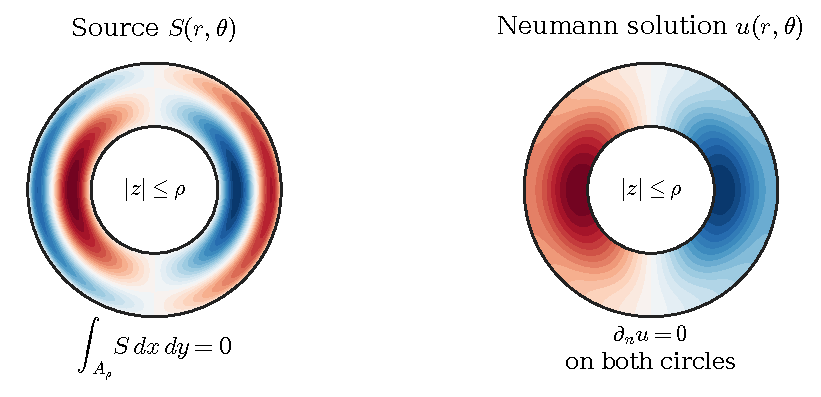
\includegraphics[width=\textwidth]{figures/output/fig06_neumann.pdf}
\caption{A scalar first-angular-mode example of the collar
construction, with colors normalized separately in the two panels.
For $x=r/\rho$, let $\chi(x)=6(x-1)^5-15(x-1)^4+10(x-1)^3$ and
$u=\rho(\chi(x)x-4x/3-4/(3x))\cos\theta$.
Then $S=-\Delta_{\RR^2}u$ has zero mean and $\partial_nu=0$
at $r=\rho,2\rho$. The matrix construction uses the same
compatibility condition and energy estimate; it does not require
this particular scalar source.}
\label{fig:neumann}
\end{figure}

Define $B=\cR(\widehat K)-D^*J$ on the whole fibre. The
component and middle-node estimates
\eqref{eq:component-residual}--\eqref{eq:transfer-residual},
the regular and radial collar estimates
\eqref{eq:regular-curvature-error}--\eqref{eq:radial-curvature-error},
and \eqref{eq:nonlinear-collar-remainder} now give
\begin{equation}\label{eq:instantaneous-b}
 \int_{C_\tau}|B|\le
 C(\alpha_*+\epsilon_*\ell^2+b^2\rho^{-N})(F+V).
\end{equation}
For the remaining Taylor terms use
$\alpha_i^2\rho^2m_i\le C\rho^2F_{\mathrm{co}}$ and
$\alpha_i^2\rho^2\ell F_{\mathrm{ed}}
\le C\alpha_*^2\rho^2\ell F_{\mathrm{ed}}$.
The time terms are bounded by $C\rho^2V$.
Thus no term weighted only by $|\alpha_i|m_i$ remains in
\eqref{eq:instantaneous-b}. Integrating
\eqref{eq:instantaneous-j} by the finite energy inequality and
\eqref{eq:instantaneous-b} by \eqref{eq:integrable-forces}
proves Proposition~\ref{prop:global-weak-residual}.

\subsection{The all-time theorem}
\begin{theorem}\label{thm:all-time}
Fix the component geometry, rank, harmonic forms, component matrices
and transports of Section~\ref{sec:geometry}. There is a radius
$R_*>0$ such that the following holds. Let the four nonzero node
parameters and the two real component parameters tend independently
to zero, and keep them fixed during each trajectory. Let $H(s)$
solve \eqref{eq:finite-flow} from $d_A(H(0),o)\le R_*$.
For any smooth determinant-normalized actual initial metric with
fixed bounds $ch_0\le h(0)\le C_0h_0$, let $h(s)$ solve HYM.
With $\widehat K$ as in Section~\ref{sec:reconstruction} and
$\eta=\int_{C_\tau}D_{\tr}(h(0),\widehat K(H(0)))$, one has
\begin{equation}\label{eq:all-time-tracking}
 \sup_{s\ge0}\int_{C_\tau}
       d(h(s),\widehat K(H(s)))^2\,dA_\tau
                     \le\eta+C a_* .
\end{equation}
The constant is independent of every scale ratio and of time.
The conclusion permits zero component weights and a nonzero
common kernel in \eqref{eq:common-kernel}. No positive lower
bound on a normalized smallest eigenvalue is assumed.
\end{theorem}

\begin{proof}
The actual flow is global and has the fixed order bounds by
\eqref{eq:order-bounds}. Its total derivative energy is bounded
by \eqref{eq:actual-energy}, since every fibre has area four.
Lemma~\ref{lem:reconstruction-energy} supplies the same bound
for the comparison. Apply Lemma~\ref{lem:weak-comparison} to the
global decomposition in Proposition~\ref{prop:global-weak-residual}.
Its right-hand side is at most $\eta+C(a_*+\rho)$, uniformly for
all finite time horizons. Since $\rho\le a_*$, taking the supremum
over horizons proves \eqref{eq:all-time-tracking}.
\end{proof}

Uniform convergence in a family of initial metrics requires
$\eta\to0$ uniformly in that family. The theorem compares each
parameter-dependent finite trajectory with its actual HYM
trajectory. It asserts neither a common limiting trajectory nor
a selected limiting phase in a nonzero kernel. When the active
constraints are irreducible, the finite limit is $o$; the theorem
still concerns absolute distance, not an error relative to the
decaying trajectory. The next section supplies an open spatial
class that enters this comparison after a negligible initial
time on every effective scale.
